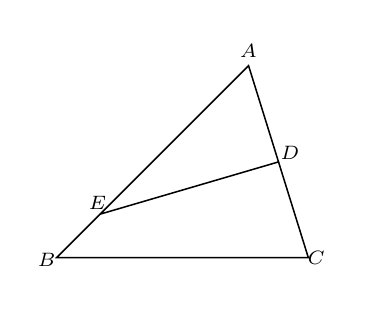
\begin{tikzpicture}[x=.023cm,y=-.023cm,baseline=(current bounding box.center),line width=.55pt,
  every node/.style={font=\scriptsize,inner sep=.8pt}]
  \path[use as bounding box] (0,0) rectangle (176,152.3);
  \coordinate (B) at (16,127);
  \coordinate (C) at (155,127);
  \coordinate (A) at (122,21);
  \coordinate (E) at (40,103);
  \coordinate (D) at (139,74);
  \draw (B)--(A)--(C)--cycle (E)--(D);
  \node[below left] at (17,123) {$B$};
  \node[below right] at (153,122) {$C$};
  \node[above] at (122,18) {$A$};
  \node[left] at (45,97) {$E$};
  \node[right] at (138,69) {$D$};
\end{tikzpicture}
